\documentclass[10pt, a4paper]{article}

\usepackage[utf8]{inputenc}
\usepackage{amsfonts}
\usepackage{amsmath}
\usepackage{amssymb}
\usepackage{vmargin}
\usepackage{mathtools}
\usepackage{enumitem}
\usepackage{cancel}
\usepackage{hyperref}
\usepackage{tikz}
\usetikzlibrary{matrix}
\usepackage{faktor}
\usepackage{tcolorbox}
\tcbuselibrary{theorems}

% Comandos útiles
\def\checkmark{\tikz\fill[scale=0.4](0,.35) -- (.25,0) -- (1,.7) -- (.25,.15) -- cycle;}
\newcommand{\R}{\mathbb{R}}
\newcommand{\N}{\mathbb{N}}
\newcommand{\Z}{\mathbb{Z}}
\newcommand{\C}{\mathbb{C}}
\newcommand{\Q}{\mathbb{Q}}
\newcommand{\F}{\mathbb{F}}
\newcommand{\eqc}[1]{\stackrel{\mathclap{\normalfont\mbox{\scriptsize{#1}}}}{=}}
\newcommand{\obs}{\underline{Observación:} }
\newcommand{\ej}{\underline{Ejemplo:} }
\newcommand{\ejs}{\underline{Ejemplos:} }
\newcommand{\nota}{\underline{Notación:} }
\newcommand{\demo}{\underline{Demostración:} }
\newcommand{\anillo}[1][]{\hyperref[def:anillo]{anillo}#1 }
\newcommand{\cuerpo}[1][]{\hyperref[def:cuerpo]{cuerpo}#1 }
\newcommand{\ideal}[1][]{\hyperref[def:ideal]{ideal}#1 }
\newcommand{\bs}{\!\!\!\!}
\newcommand{\longhookrightarrow}{\lhook\joinrel\longrightarrow}

\definecolor{royalfuchsia}{rgb}{0.79, 0.17, 0.57}

\newenvironment{enumerater}{\begin{enumerate}[label=\roman*)]}
{\end{enumerate}}
\newenvironment{enumeratea}{\begin{enumerate}[label=\arabic*)]}
{\end{enumerate}}

\tcbset{
	% Definición de estilos de recuadros
	defstyle/.style={colback=blue!5, colframe=blue!85!black, before={\vspace{5mm}}, after={\vspace{5mm}}}, % Definiciones
	theostyle/.style={colback=red!5, colframe=red!80!black, before={\vspace{5mm}}, after={\vspace{5mm}}}, % Teoremas
	propstyle/.style={colback=green!5, colframe=green!60!black, before={\vspace{5mm}}, after={\vspace{5mm}}}, % Proposiciones
	corstyle/.style={colback=green!5, colframe=royalfuchsia, before={\vspace{5mm}}, after={\vspace{5mm}}} % cor
}

% Definicion de las cajas
\newtcbtheorem[number within=section]{definition}{Definición}{defstyle}{def}
\newtcbtheorem[number within=section]{theorem}{Teorema}{theostyle}{theo}
\newtcbtheorem[number within=section]{proposition}{Proposición}{propstyle}{prop}
\newtcbtheorem[number within=section]{corolary}{Corolario}{corstyle}{cor}

\setlength{\parindent}{0pt}
\setmargins{2.5cm}       % margen izquierdo
{1.5cm}                        % margen superior
{16cm}                      % anchura del texto
{23.42cm}                    % altura del texto
{10pt}                           % altura de los encabezados
{1cm}                           % espacio entre el texto y los encabezados
{0pt}                             % altura del pie de página
{2cm}

\begin{document}

\title{Teoría de Galois}
\author{Carlos Gómez-Lobo}
\date{}
\maketitle


\section{Anillos}

A continuación vamos a repasar algunos conceptos sobre anillos y especialmente anillos de polinomios, empezando por la definición de anillo.

\begin{definition}{Anillo}{anillo}
Un \textbf{anillo} es un conjunto no vacío dotado de dos operaciones, que denotaremos como suma (+) y multiplicación ($\cdot$) y que cumplen las siguientes propiedades:
\begin{itemize}
	\item $(R, +)$: grupo abeliano
	\item $(R, \cdot)$: operación binaria interna y cumple la propiedad asociativa
\end{itemize}
Si además $(R, \cdot)$ tiene identidad, es decir, existe un elemento $e \in R$ tal que $e \cdot r = r \cdot e = r \; \forall r \in R$, diremos que $R$ es un anillo con unidad y si además es abeliano, entonces será un anillo conmutativo.
\end{definition}

A nosotros en esta asignatura nos interesarán especialmente estos últimos y nos referiremos a estos simplemente como anillos sin especificar que son conmutativos y sin unidad.

\vspace{3mm}

\underline{Ejemplos:} $\Z, \Z_n, \R, \C, \Q, M_n(\R)$ (no conmutativo), etc.

\vspace{3mm}

\underline{Notación:} \begin{itemize}
	\item 0 para el elemento neutro de la suma
	\item $-a$ para el elemento inverso aditivo (opuesto).
	\item 1 para el elemento neutro de la multiplicación
	\item $a^{-1}$ para el inverso multiplicativo, si existe
	\item $na = \underbrace{a + ... + a}_{\text{n veces}}$
	
	\vspace{-3mm}
	
	\item $a^n = \underbrace{a \cdot ... \cdot a}_{\text{n veces}}$
\end{itemize}

\begin{definition}{Cuerpo}{cuerpo}
Un anillo $(R, +, -)$ es un \textbf{cuerpo} si $(R^* = R \backslash \{0\}, \cdot)$ es un grupo abeliano.
\end{definition}

\underline{Ejemplos:} $\Q, \R, \C, \Z_p$ p primo, etc.

\vspace{3mm}

\underline{Notación:} $\; \Z_n  \left \{
\begin{matrix*}[l]
\textrm{grupo aditivo} \rightarrow \C_n \\
\textrm{anillo} \rightarrow \Z_n \\
\textrm{cuerpo} \rightarrow \mathbb{F}_n \textrm{(n primo)}
\end{matrix*} \right .$

\begin{definition}{Divisor de cero}{div_cero}
Sea $R$ un anillo. Diremos que un elemento $a \in R, \; a \neq 0$ es un \textbf{divisor de cero} si $\exists b \in R, \; b \neq 0$ tal que $a \cdot b = 0$.
\end{definition}

\ej En $\Z_6: \bar{2}, \bar{3} \neq \bar{0}$ y $\bar{2} \cdot \bar{3} = 0$.

\begin{definition}{Dominio de integridad}{DI}
Sea $R$ un anillo, si $R$ no tiene divisores de cero, entonces se dice que es un \textbf{dominio de integridad}.
\end{definition}

\ejs $\Z, \Q, \R, \C, \F_p$

\begin{definition}{"Divide a"}{dividea}
Diremos que $a$ \textbf{divide a} $b$ en $R$ si $\exists c \in R$ tal que $b = a \cdot c$ y escribiremos $a | b$.
\end{definition}

\subsection{Subanillos}

\vspace{3mm}

\begin{definition}{Subanillo}{subanillo}
Diremos que $S \subset R$ es un \textbf{subanillo} si $(S, +, \cdot)$ es un anillo.
\end{definition}

\obs $S \subset R$ es un subanillo s y solo si:

\begin{enumerate}[label=\arabic*)]
	\item $S \neq \emptyset$
	\item $\forall a, b \in S, a + b \in S$
	\item $\forall a, b \in S, a \cdot b \in S$
	\item $1 \in S$
\end{enumerate}

\vspace{3mm}

\ej $\Z \subset \Q \subset \R \subset \C$

\begin{definition}{Menor subanillo que contiene a un elemento}{menoranillo}
Dado un anillo $R$ y un elemento $a$, podemos definir el \textbf{menor subanillo que contiene a $\mathbf{R}$ y al elemento $\mathbf{a}$} como $R[a] = \left \{ \displaystyle\sum r_i \cdot a^k, \forall r \in R; i, k \in \N \right \}$
\end{definition}

\ej $\Z[i] = \{a + bi, a, b \in \Z\} \subset \C$. Otra forma de ver este anillo es como la intersección de todos los subanillos de $\C$ que contienen a $\Z$ y a $i$.

\vspace{3mm}

\obs De la misma forma podemos definir el menor cuerpo que contiene a un elemento y que denotamos como $R(a)$.

\vspace{3mm}

\ej $\Q[\sqrt{2}] = \{a + b\sqrt{2}, \; a, b \in \Q\}$, $\Q(\sqrt{2}) = \bigg \{ \dfrac{a + b\sqrt{2}}{\underbrace{c + d\sqrt{2}}_{\neq 0}}, \; a, b, c, d \in \Q \bigg \}$, $\Q \subset \Q[\sqrt{2}] \subset \Q(\sqrt{2}) \subset \R$

\subsection{Anillos de polinomios}

\vspace{3mm}

\begin{definition}{Anillo de polinomios}{anillopoli}
Sea $R$ un anillo, llamaremos a $R[x]$ al \textbf{anillo de polinomios con coeficientes en $\mathbf{R}$} y que será de la forma $R[x] = \left \{ \displaystyle\sum_{k = 0}^{n} r_k x^k, \; \forall r \in R \right \}$.
\end{definition}

\ejs $\C[x], \R[x], \Q[x], \Z[x]$, etc.

\begin{definition}{Coeficiente director}{coef_dir}
El \textbf{coeficiente director} de un polinomio es el coeficiente distinto de 0 que multiplica a la x de mayor grado.
\end{definition}

\nota Grado de $p(x) := deg(p(x))$

\vspace{3mm}

\begin{proposition}{}{grado_prod}
El grado del producto de dos polinomios puede tener distintos valores en función de si el anillo sobre el que se construye es o no un \hyperref[def:DI]{DI}:
\[
deg(p(x) \cdot q(x)) = \left \{
\begin{matrix*}[l]
deg(p(x)) + deg(q(x)) \text{ si $R$ \hyperref[def:DI]{es dominio de integridad}} \\
\leq deg(p(x)) + deg(q(x)) \text{ si no lo es}
\end{matrix*} \right .
\]
\end{proposition}

\demo Obvio.

\vspace{3mm}

\ej $\Z_4, \left .
\begin{matrix*}[l]
p(x) = 2x + 1 \\
q(x) = 2x
\end{matrix*} \right \}
deg(p(x) \cdot q(x) = 1 < 2$

\vspace{3mm}

\begin{proposition}{}{grado_DI}
 Sea $R$ un \hyperref[def:cuerpo]{cuerpo}, entonces $R$ es siempre \hyperref[def:DI]{dominio de integridad} y para cualesquiera polinomios de $R[x]$ se cumple que $deg(p(x)) \cdot deg(q(x)) = deg(p(x)) + deg(q(x))$.	
\end{proposition} 
 
\demo Para demostrar que un cuerpo siempre es un \hyperref[def:DI]{DI} vamos a ver por reducción al absurdo que todo elemento de un anillo que tenga inverso multiplicativo no es \hyperref[def:div_cero]{divisor de cero}.

Suponemos que $r \neq 0 \in R$ es \hyperref[def:div_cero]{divisor de cero}, es decir, $\exists r^{-1}$ tal que $r' \neq 0, r \cdot r' = 0$. Ahora suponemos además que $r$ es invertible, es decir, $\exists r^{-1}$ tal que $r \cdot r^{-1} = 1$. Entonces $r \cdot r^{-1} = 1 \implies (r' \cdot r) \cdot r^{-1} = b \implies 0 = b$. Contradicción.

De la misma forma se puede ver que una unidad no puede ser un \hyperref[def:div_cero]{divisor de cero} y como en un cuerpo todos sus elementos son unidades, no hay ningún \hyperref[def:div_cero]{divisor de cero} y por tanto es un \hyperref[def:DI]{dominio de integridad}.

Por esto y por la proposición \ref{prop:grado_prod}, queda demostrado.

\begin{proposition}{}{apoli_nocuerpo}
Sea $K$ un cuerpo, entonces el anillo de polinomios asociado a $K, \; K[x]$  \textbf{no} es un cuerpo y sus únicos elementos invertibles son los pertecientes al cuerpo $K$ no nulos.
\end{proposition}

\demo Sea $p(x) \in K[x], \; p(x) \neq 0$ invertible en $K[x]$. Entonces $p(x) \cdot p^{-1}(x) = 1, \; deg(1) = 0$ y como por la proposición \ref{prop:grado_prod}, $deg(p(x) \cdot p^{-1}(x)) \leq deg(p(x)) + deg(p^{-1}(x))$, se tiene que $deg(p(x)) = deg(p^{-1}(x)) = 0$, por lo que los únicos elementos invertibles en $K[x]$ son los de grado 0, que son los no nulos que pertenecen a $K$. Entonces, puesto que no todos los elementos de $K[x]$ son invertibles, $K[x]$ no es un cuerpo.

\vspace{3mm}

\obs El menor cuerpo que contiene a x y a los elementos de $K$ es \\ $K(x) = \left \{ \dfrac{p(x)}{q(x)} : p(x), q(x) \in K[x], q(x) \neq 0 \right \}$, teniendo en cuenta que $\dfrac{p(x)}{q(x)} = \dfrac{p'(x)}{q'(x)} \iff p(x) q'(x) = p'(x) q(x)$.

\begin{definition}{Polinomio mónico}{poli_mon}
Un \textbf{polinomio mónico} es aquel cuyo \hyperref[def:coef_dir]{coeficiente director} es 1.
\end{definition}

\subsection{Ideales en un anillo}

\vspace{3mm}

\begin{definition}{Ideal}{ideal}
Sea $R$ un anillo. Un \textbf{ideal} en $R$ es un subconjunto no vacío $I \subset R$ tal que:
\begin{enumerate}[label=\roman*)]
	\item $(I, +)$ es un subgrupo de $R$.
	\item $\forall r \in R, \; \forall a \in I, \; r \cdot a \in I$ (Propiedad de absorción).
\end{enumerate}
\end{definition}

\begin{proposition}{Criterio para ideales}{crit_ideal}
Para que un subanillo $I \subset R, \; I \neq \emptyset$ sea un ideal tiene que cumplir que:

\begin{enumerate}[label=\roman*)]
	\item $\forall a, b \in I, \; a - b \in I \; (a + b \in I)$.
	\item $\forall r \in R, \; \forall a \in I, \; r \cdot a \in I$.
\end{enumerate}
\end{proposition}

\ejs
\begin{enumerate}[label=\arabic*)]
	\item $R$ anillo cualquiera
		\begin{enumerate}[label=\roman*)]
			\item $R$ es un ideal (el ideal trivial).
			\item \{0\} siempre es un ideal.
		\end{enumerate}

Si $I \subset R$ es un ideal e $I \neq R$, diremos que $I$ es un \textbf{ideal propio}.

	\item En $\Z$ todos los anillos de la forma $I = \{2n : n \in \Z\}$ son ideales.
	
	\item $\Q[x], \; I = \{p(x) : p(r_0) = 0, \; r_0 \in \Q \}$
			
			Comprobación: Sean $p(x), q(x), t(x) \in \Q[x]$ tal que $p(r_0) = q(r_0) = 0,  \; t(x)$ cualquiera, entonces:
		\begin{enumerater}
			\item $s(r_0) = p(r_0) - q(r_0) = 0 \implies s(x) \in I$.
			\item $z(r_0) = p(r_0) \cdot t(r_0) = 0 \implies z(x) \in I$.
		\end{enumerater}
	\item 
\end{enumerate}

\begin{proposition}{}{ideales_z}
Todos los ideales de $\Z$ son de la forma $\{kn : n \in \Z\}$.
\end{proposition}

\demo Sale del algoritmo de la división.

\vspace{5mm}

\obs Sea $R$ un anillo y sean $I, J \subset R$ ideales, entonces:

\begin{enumerater}
	\item En general, $I \cup J$ \textbf{no} es un ideal.
	\item $I \cap J$ es un ideal
\end{enumerater}

\begin{proposition}{}{ideales_cuerpo}
Sea $K$ un anillo, entonces $K$ es un \hyperref[def:cuerpo]{cuerpo} si y solo si continene dos \hyperref[def:ideal]{ideales}: $\{0\}$ y $K$.
\end{proposition}

\demo 

$\implies$) Sea $I \in K, \; I \neq \{0\}$ un ideal y $r \in I, \; r \neq 0$ uno de sus elementos. Por ser $K$ un cuerpo $\exists r^{-1}$ tal que $r \cdot r^{-1} = 1 \in I$ (Propiedad de absorción) $\implies I = K$.

$\impliedby$) Sea $K$ un anillo y $r \in K, \; r \neq 0$. Vamos a ver que $r$ tiene un inverso.

Definimos $I := \{rs : s \in K\}$ que es un ideal. Puesto que $I \neq \{0\}$ y solo hay dos ideales, $I = K \implies 1 \in K \implies \exists s \in K$ tal que $s \cdot r = 1 \implies s = r^{-1}$.

\begin{definition}{Ideal generado}{ideal_generado}
Sea $R$ un \anillo y $\{r_i\}$ una familia de elementos de $R$. Diremos que el \textbf{ideal generado} por $\{r_i\}_{i \in I}$ es el ideal más pequeño que contiene a $\{r_i\}_{i \in I}$ y lo denotamos por $\langle r_i \rangle_{i \in I} = \left \{ \displaystyle\sum s_j r_i : s_j \in R \right \}$.
\end{definition}

\ej En $\Z[x]$ el ideal generado por $\langle 2, x \rangle = \{2q(x) + xp(x)\ : q(x), p(x) \in \Z\}$

\begin{definition}{Ideal principal}{ideal_principal}
Sea $R$ un \anillo, diremos que $I \subset R$ es un \textbf{ideal principal} si $\exists a \in R$ tal que $I = \langle a \rangle$.
\end{definition}

\ej
\begin{enumeratea}
\item En $\Z$ todos los ideales son principales.
\item $\langle 2, x \rangle \subset \Z[x]$ no es principal.

Comprobación: Suponemos que $\exists g(x) \in \Z[x]$ tal que $\langle 2, x \rangle = \langle g(x) \rangle$, entonces $\exists q(x)$ tal que $g(x) \cdot q(x) = 2 \implies deg(g(x)) = 0 \implies g(x) = k \in \Z \implies k = \pm 1, \pm 2$

Supongamos que $k = \pm 1$. Entonces $\langle g(x) \rangle = \langle \pm 1 \rangle = \langle 2, x \rangle = \Z[x]$. Sin embargo, $1 = \underbrace{2p(x)}_{\text{coef. par}} + \cancelto{0}{\underbrace{q(x)x}_{grado \geq 1}}$. Contradicción.

Ahora si suponemos que $k = \pm 2 \implies \langle g(x) \rangle = \langle \pm 2 \rangle = \langle 2, x \rangle =$ polinomios con coeficientes pares, pero $x \notin \langle \pm 2 \rangle$. Contradicción.
\end{enumeratea}

\begin{definition}{Dominio de ideales principales (DIP)}{DIP}
Sea $R$ un \anillo{,} si todos los \hyperref[def:ideal]{ideales} contenidos en $R$ con principales se dice que es un \textbf{dominio de ideales principales}.
\end{definition}

\begin{proposition}{}{cuerpo_ideal_ppal}
Sea $K$ un \cuerpo entonces $K[x]$ es un \hyperref[def:DIP]{dominio de ideales principales}.
\end{proposition}

\demo Sea $I \subset K[x]$ un ideal.
\begin{itemize}
\item Si $I = \{0\}$ \checkmark
\item Suponemos que $I \neq \{0\} \implies \exists p(x) \in I, \; p(x) \neq 0$ y podemos definir $\Lambda = \{deg(p(x)) : p(x) \in I\} \neq \emptyset, \; \Lambda \subset \N$. Por la propiedad de buen orden de $\N$ podemos afirmar que $\Lambda$ tiene un elemento mínimo $n$, por lo que $\exists p(x) \in I$ tal que $deg(px) = n$ y además $\langle p(x) \rangle \subseteq I$. Ahora vamos a demostrar por el algoritmo de la división de polinomios que $\langle p(x) \rangle = I$.

Sea $s(x) \in I \implies s(x) = q(x)p(x) + r(x)$ y hay dos posibilidades para $r(x)$:
	\begin{itemize}[label=$\circ$]
		\item $r(x) = 0 \implies p(x) \mid q(x) \; \checkmark$
		\item $r(x) \neq 0, \; \underbrace{s(x)}_{\in I} = \underbrace{q(x) \underbrace{p(x)}_{\in I}}_{\in I} + r(x) \overset{Prop. 1}{\implies} r(x) \in I$. Contradicción porque $deg(r(x)) < deg(p(x))$ que es el grado mínimo en $I$.
	\end{itemize}
\end{itemize}

\ej Usando un argumento similar con el algoritmo de la división en $\Z$ se puede probar que este es un \hyperref[def:DIP]{DIP}.

\vspace{5mm}

\obs El generador de un ideal $I \subset K[x]$ no tiene por qué ser único: si $I = \langle p(x) \rangle$ y $a \in K$, entonces $I = \langle ap(x) \rangle$. Para describir estos anillos de forma canónica utilizaremos como generador un \hyperref[def:poli_mon]{polinomio mónico}.

\subsection{Anillos cociente}

\vspace{3mm}

\begin{definition}{Anillo conciente}{anillo_conciente}
Sea $I \subset R$ un ideal en $R$, podemos definir como en los grupos al conjunto $\faktor{R}{I}$ como el \textbf{anillo cociente} según la relación de equivalencia $a = b \iff a - b \in I$.
\end{definition}

Ahora vamos a comprobar algunas cosas sobre la definición anterior:

\begin{enumerate}
	\item La relación de equivalencia usada es realmente una relación de equivalencia estudiando sus tres propiedades:
	\begin{enumerater}
		\item Reflexiva: $a - a = 0 \in I$ \checkmark
		\item Simétrica: $a = b \implies a - b \in I \implies (a - b) \cdot -1 \in I \implies (b - a) \in I \implies b = a$ \checkmark
		\item Transitiva: $a = b$ y $b = c \implies a - b \in I$ y $b - c \in I \overset{\text{Prop. 1}}{\implies} a - b + b -c = a - b \in I \implies a = c \;$\checkmark
	\end{enumerater}
	\item El conjunto cociente resultado tiene estructura de anillo. Para ello solo es necesario comprobar que el producto está bien definido, es decir, de dos elementos no depende del representante escogido.
	
	Sean $\bar{a} = \{a + I\}, \bar{b} = \{b + I\}$, entonces $(a + I)(b + I) = ab + \overbrace{\underbrace{aI}_{\in I} + \underbrace{bI}_{\in I} + I}^{\in I} = ab + I \implies \bar{a}\bar{b} = \overline{ab} \;$\checkmark
\end{enumerate}

		
\obs 
\begin{enumerate}
	\item Si el anillo $R$ es conmutativo y con unidad, entonces $\faktor{R}{I}$ tamibién lo es y su unidad es $\bar{1}$.
	\item $\forall a \in I, \; \bar{c} = 0$.
\end{enumerate}

\ejs 
\begin{enumeratea}
	\item $\faktor{\Z}{n\Z} = \Z_n$
	\item $\faktor{R}{R} = \{0\}$
	\item $\faktor{R}{\{0\}} = R$
	\item $S = \faktor{\R[x] \;}{\langle x^2 + 1 \rangle}$: ¿Qué pinta tiene? En primer lugar, vamos a comprobar que todo elemento de $S$ es equivalente a un elemento de la forma $ax + b, \; a, b \in \R$.
	Sea $p(x) \in \R[x]$, ¿$\overline{p(x)}$? $p(x) = q(x)(x^2 + 1) + r(x)$ donde $r(x) = 0$ ó $deg(r(x)) \leq 1 \implies p(x) - r(x) \in \langle x^2 + 1 \rangle \implies \overline{p(x)} = \overline{r(x)}$.
\end{enumeratea}


\subsection{Homomorfismos de anillos}

\vspace{3mm}

\begin{definition}{Homomorfismo de anillos}{homomorfismo}
Sean $R$ y $T$ anillos. Un \textbf{homomorfismo de anillos} $f : R \longrightarrow T$ es una función que verifica las siguientes propiedades:

\begin{enumerater}
	\item $f(r + r') = f(r) + f(r'), \; \forall r, r' \in R$
	\item $f(r \cdot r') = f(r) \cdot f(r'), \; \forall r, r' \in R$
	\item (Homomorfismo de anillos unitarios) $f(1_R) = 1_T$
\end{enumerater}

\obs Nosotros siempre utilizaremos homomorfismos de anillos unitarios y nos referiremos a ellos simplemente como homomorfismos.

\end{definition}

\ejs 
\begin{enumeratea}
	\item Con este ejemplo vamos a comprobar cuántos homomorfismos existen de $\Z$ en $\Z$.
	Si utilizamos las propiedades vistas anteirormente, tenemos que $1 \longrightarrow 1 \overset{\text{Prop. 1}}{\implies} n = \underbrace{1 + \cdots + 1}_{\text{n veces}} \longrightarrow f(n) = \underbrace{f(1) + \cdots f(1)}_{\text{n veces}} \implies f = Id$
	\item Sea $R$ un anillo cualquiera:
	\[
	\begin{matrix*}[l]
		f : \Z &\bs\longrightarrow &\bs R \\
		\hspace{5mm} 1 &\bs\longrightarrow & \bs1_R \\
		\hspace{5mm} n &\bs\longrightarrow &\bs f(n) = \underbrace{1_R + \cdots 1_R}_{\text{n veces}}
	\end{matrix*}
	\]
	Un caso especial de este tipo es cuando $p \in \Z$ es un primo y $f(p) = 0_R$, entonces la función:
	\[
		\begin{array}{cl}
			\bar{F} : R &\bs\longrightarrow R \\
			\hphantom{F :} a &\bs\longrightarrow a^p
		\end{array}
	\]
	Es un homomorfismo de anillos llamado el "homomorfismo de frobenius" \label{homo_frobenius} y cumple que en $R, \; {(a + b)}^p = a^p + b^p$.
	
	\item En este comprobaremos si existe algún homomorfismo de $\Z[i]$ en $\Z[\sqrt{2}]$:
	\[
	\begin{matrix}
		f : \Z[i] &\bs\longrightarrow& \bs\Z[\sqrt{2}] \\
		\hphantom{f :} 1 &\bs\longrightarrow& \bs\bs1 \\
		n \in \Z & \bs\longrightarrow& \bs n \in \Z
	\end{matrix}
	\]
	La función $f$ mandará al elemento $i$ a un elemento de $\Z[\sqrt{2}]$ de la forma $a + b\sqrt{2}$, sin embargo: 
	\[f(i^2) = \left \{
	\begin{matrix*}[l]
		{f(i)}^2 = {(a + b\sqrt{2})}^2 \geq 0\\
		f(-1) = -1
	\end{matrix*} \right . \implies \text{Contradicción}
	\]
	\item Sea $\Z[x]$ el anillos de polinomios con coeficientes enteros y $T$ un anillo cualquiera:
	\[
	\begin{array}{rl}
		f : \Z[x] &\bs\longrightarrow T \\
		x\;\; &\bs\longrightarrow t \in T \\
		p(x) &\bs\longrightarrow p(t)
	\end{array}
	\]
\end{enumeratea}

\begin{proposition}{Propiedades de los homomorfismos de anillos}{prop_homomorfismos}
	Sea $f : R \longrightarrow T$ un \hyperref[def:homomorfismo]{homomorfismo de anillos}:
	\begin{enumeratea}
		\item Si $S \in R$ es un subanillo, entonces $f(S) \in T$ es un subanillo
		\item Si $J \in T$ es un ideal, entonces $f^{-1}(J)$ es un ideal de $R$.
		\item Si $f$ es sobreyectivo e $I \in R$ un ideal, entonces $f(I)$ es un ideal en $T$.
		\item $Ker\ f = f^{-1}(\{0\})$ es un ideal en $R$.
		\item $f$ es inyectivo $\iff Ker\ f = \{0\}$.
	\end{enumeratea}
\end{proposition}

\demo 
\begin{enumeratea}
	\item Por las propiedades de homomorfismos $f(S)$ es un grupo aditivo y el producto es interno y asociativo.
	\item Teniendo que $\forall s_1, s_2 \in f^{-1}(J), \; \exists t_1, t_2 \in J$ tal que $s_1 = f^{-1}(t_1), s_2 = f^{-1}(t_2)$, vamos a comprobar que cumple las propiedades de un ideal:
	\begin{enumerater}
		\item $\underbrace{t_1 - t_2}_{\in f^{-1}(J)} = f(s_1) - f(s_2) = f(s_1 - s_2) \in f^{-1}(J) \implies s_1 - s_2 \in J$
		\item $\forall t \in T,\ t_1 \cdot t \in f^{-1}(J) \implies \exists r \in R$ tal que $f(r) = t_1 \cdot t = f(s_1) - t \implies t = f(\underbrace{r - s_1}_{r'}) \implies t_1 \cdot t = f(s_1 \cdot s') \in f(J) \implies s_1 \cdot s' \in J$
	\end{enumerater}
	\item Como $f$ es sobreyectivo, podemos afirmar que $\forall t \in T, \;\exists r \in R$ tal que $f(r) = t$ y teniendo $t_1, t_2 \in f(I)$ tal que $t_1 = f(s_1), t_2 = f(s_2),\; s_1, s_2 \in I$ entonces:
	\begin{enumerater}
		\item $t_1 - t_2 = f(s_1) - f(s_2) = f(\underbrace{s_1 - s_2}_{\in I}) \in f(I)$
		\item $t_1 \cdot t \ \eqc{sobre} \  f(s_1) \cdot f(s) = f(\underbrace{s_1 \cdot s)}_{\in I} \in f(I)$
	\end{enumerater}
	\item Comprobamos una vez más que cumple las propiedades de un ideal teniendo $s_1, s_2 \in Ker\ f$:
	\begin{enumerater}
		\item $f(s_1 - s_2) = f(s_1) - f(s_2) = 0 \implies s_1 - s_2 \in Ker\ f$
		\item $\forall r \in R,\ f(s_1 \cdot r) = f(s_1) \cdot f(r) = 0 \cdot f(r) = 0 \implies s_1 \cdot r \in I$
	\end{enumerater}
	\item Vamos a demostrar ambas implicaciones: \\
	\indent $\implies )$ Es obvio que la antiimagen del $0_T$ es el $0_S$, y por ser inyectiva es el único.

	\indent \ $\Longleftarrow\ )$ Vamos a demostrarlo por reducción al absurdo. Supongamos que $f$ no es inyectiva, es decir, $\exists r_1, r_2 \in R,\ r_1 \neq r_2$ tal que $f(r_1) = f(r_2) = t, t \in T$, entonces:
	\[
	f(r_1 - r_2) = f(r_1) - f(r_2) = t - t = 0 \implies r_1 - r_2 \in Ker\ f \implies r_1 - r_2 = 0 \implies r_1 = r_2 \implies \text{Contradicción}
	\]
\end{enumeratea}
\obs Si $I \in R$ es un ideal, en general $f(I) \in T$ \emph{no} es un ideal.

\begin{corolary}{}{homo_cuerpo_inyectivo}
Sea $K$ un \cuerpo y $f : K \longrightarrow T$, entonces $f$ es necesariamente inyectivo.
\end{corolary}

\demo Como $Ker\ f$ es un ideal en $K$ y este es un cuerpo, entonces por la proposición \ref{prop:ideales_cuerpo} $Ker\ f$ tiene que ser o bien $K$, que no puede ser porque $1_K$ no iría a $1_T$, o bien $\{0\}$, por lo que es inyectivo.

\vspace{3mm}

\obs Si $f : R \longrightarrow T$ es un homomorfismo de anillos biyectivo, entonces su inverso $f^{-1} : T \longrightarrow R$ es un homomorfismo de anillos. Por tanto, todo homomorfismo de anillos biyectivo es un isomorfismo.

\begin{theorem}{1$^{\text{er}}$ Teorema de isomorfía}{iso_1}
Sea $f : R \longrightarrow T$ es un \hyperref[def:homomorfismo]{homomorfismo de anillos}, entonces:
\begin{enumeratea}
	\item Existe un homomorfismo de anillos $\bar{f}$ de $\faktor{R}{Ker\ f}$ en $T$ que está bien definido tal que $\forall r \in R,\ \bar{f}(\bar{r}) := f(r)$.

	\vspace{-5mm}

	\begin{center}
		\begin{tikzpicture}
			\matrix (m) [matrix of math nodes,row sep=3em,column sep=4em,minimum width=2em] {
			R & T \\
			\faktor{R}{Ker\ f} & \\
			};
			\path[-stealth]
				(m-1-1) edge node [above] {f} (m-1-2)
						edge (m-2-1)
				(m-2-1) edge node [below] {$\bar{f}$} (m-1-2);
		\end{tikzpicture}
	\end{center}
	\item $\bar{f}$ es inyectivo y por tanto hay un isomorfismo:
	\[
	\faktor{R}{Ker\ f} \simeq f(R) \in T
	\]
	
\end{enumeratea}
\end{theorem}

\subsection{Característica de un anillo}

\vspace{3mm}

Sea $R$ un anillo cualquiera y $f$ un homomorfismo de $\Z$ en $R$, entonces se tiene que $Ker\ f \in \Z$ es un ideal pero, ¿cómo son los ideales de $\Z$?
\begin{enumerate}[label=\alph*)]
	\item $Ker\ f = \{0\} \implies \Z \longhookrightarrow R$, es decir, $\Z$ es un subanillo de $R$.
	\item $ker\ f = \langle n \rangle,\ n \neq 0$
\end{enumerate}

Utilizando el \hyperref[theo:iso_1]{primer teorema de isomorfía} podemos ver que $\faktor{\Z}{n\Z} \longhookrightarrow R$, por lo que podemos pensar que $\Z_n$ es un subanillo de $R$. Con esto llegamos a la siguiente definición:

\begin{definition}{Característica de un anillo}{caracter}
Sea $R$ un \anillo y $f$ un \hyperref[def:homomorfismo]{homomorfismo de anillos} de $\Z$ en $R$, entonces definimos la \textbf{característica de un anillo} como:
\[
char(R) = \left \{
\begin{matrix*}[l]
	0 \text{ si } Ker\ f = 0 \\
	n \text{ si } ker\ f = \langle n \rangle
\end{matrix*} \right .
\]

Otro modo de definir $char(R)$, es decir que es el orden de $1_R$ como elemento de $(R, +)$. Si el orden de $1_R$ no es finito, entonces decimos que $char(R) = 0$.
\end{definition}

\nota Cuando decimos por ejemplo que $\Z \subset R$ o alguno de sus conjuntos cocientes en realidad hacemos una abuso de lenguaje y a lo que nos referimos es a que existe un anillo $S$ tal que $\Z \simeq S \subset R$.

\vspace{3mm}


\obs Volviendo al ejemplo del homomorfismo de Frobenius, se tiene que si $char(R) = p$, entonces la función
$\arraycolsep=1pt
\begin{array}{rcl}
	R & \overset{F}{\longrightarrow} & R \\
	a & \longrightarrow & a^p
\end{array}
$ es un homomorfismo de anillos.

\ejs
\begin{enumeratea}
	\item $char(\Z) = 0$
	\item $char(\Q) = 0$ (inyectivo)
	\item $char(\R) = char(\C) = 0$
	\item $char(\Z_n) = n
	\left (\arraycolsep=1pt
	\begin{array}{ccl}
		\Z & \longrightarrow & \Z_n = \faktor{\Z}{n\Z} \\
		1 & \longrightarrow & \bar{1}
	\end{array}
	\right )$
	\item $char(R) = char(R[x])\ \ 
		\left (\arraycolsep=1pt
		\begin{array}{rcccl}
			\Z & \longrightarrow & R & \longhookrightarrow & R[x] \\
			1 & \longrightarrow & 1_R & \longrightarrow & 1_R
		\end{array}
		\right)$
	\item Sea $R = \Z \times \Z_5$ con las operaciones coordenada a coordenada, $char(R) = 0\ \ 
	\left (\arraycolsep=1pt
	\begin{array}{ccc}
		\Z & \longrightarrow & \Z \times \Z_5 \\
		1 & \longrightarrow & (1, \bar{1})
	\end{array}
	\right )$
\end{enumeratea}

\begin{proposition}{Característica de un dominio de integridad}{carac_DI}
Sea $R$ un \hyperref[def:DI]{dominio de integridad}, entonces la \hyperref[def:caracter]{característica} de $R$ será $0$ o prima.
\end{proposition}

\demo Por el \hyperref[theo:iso_1]{primer teorema de isomorfía}, tenemos que:
\begin{center}
	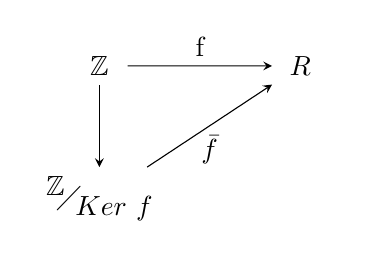
\begin{tikzpicture}
		\matrix (m) [matrix of math nodes,row sep=3em,column sep=4em,minimum width=2em] {
		\Z & R \\
		\faktor{\Z}{Ker\ f} & \\
		};
		\path[-stealth]
			(m-1-1) edge node [above] {f} (m-1-2)
					edge (m-2-1)
			(m-2-1) edge node [below] {$\bar{f}$} (m-1-2);
	\end{tikzpicture}
\end{center}

Entonces, $\faktor{\Z}{Ker\ f} = \faktor{\Z}{n\Z} \subset R$ y como $\bar{f}$ es inyectiva y $R$ un DI, $\Z_n$ tiene que ser también un DI, por lo que $n$ solo podrá ser primo o $0$.

\begin{corolary}{Característica de un cuerpo}{caracter_cuerpo}
Sea $K$ un \cuerpo, entonces su característica será $0$ o prima.
\end{corolary}

\demo Resultado directo pues todo cuerpo es un DI.

\begin{proposition}{}{ideales_y_homo}
Sea $R$ un \anillo, $I \subset R$ un \hyperref[def:ideal]{ideal} y $\pi$ una función de la forma:
\[\arraycolsep=2pt
\begin{array}{ccl}
	R & \overset{\pi}{\longrightarrow} & \faktor{R}{I} \\
	a & \longrightarrow & \bar{a}\ mod(I)
\end{array}
\]
Entonces $\pi$ es un \hyperref[def:homomorfismo]{homomorfismo de grupos} y se tiene que:

\begin{enumerate}
	\item Si $\pi$ es sobreyectivo y $J \subset R$ un ideal, entonces $\pi(J) \subset \faktor{R}{I}$ es un ideal.
	\item Si $a \in R$ entonces $\pi(a) = \pi(a + I)$.
	\item Si $J \subset R$ es un ideal, entonces $\pi(J) = \pi(J + I)$, siendo $J + I$ el ideal más pequeño que contiene a $J$ y a $I$.
	\item Sea $L \subset \faktor{R}{I}$ un ideal, entonces $\pi^{-1}(L)$ es un ideal en $R$ y además $I \subset \pi^{-1}(L)$.
	\item Sean $J_1,\ J_2 \subset R$ ideales tal que $I \subset J_1 \subsetneq J_2$ entonces $\pi(J_1) \subsetneq \pi(J_2)$.
\end{enumerate}
\end{proposition}

\demo Vamos a demostrar el punto 5. Está claro que $\pi(J_1) \subset \pi(J_2)$ pero, ¿cómo sabemos que son distintos? Lo comprobamos por redicción al absurdo. Para ello supondremos que $\pi(J_1) = \pi(J_2)$, por lo que $\exists a \in J_2 \setminus J_1,\ b \in J_1$ tal que $\pi(a) = \pi(b)$. Enotnces $\underbrace{a}_{\in J_2 \setminus J_1} = \underbrace{\underbrace{b}_{\in J_1} + \underbrace{r}_{\in I \subset J_1}}_{\in J_1}$. Contradicción.

\begin{theorem}{Correspondencia biyectiva}{corr_biy}
Sean $R$ un \anillo, $I \in R$ un \hyperref[def:ideal]{ideal} y $\pi$ un \hyperref[def:homomorfismo]{homomorfismo} de $R$ en $\faktor{R}{I}$, entonces se tiene que existe una \textbf{correspondencia biyectiva} entre los ideales de $R$ que contienen a $I$ y los ideales de $\faktor{R}{I}$.
\end{theorem}

\demo Se deja como ejercicio para el lector.

\vspace{3mm}

\ejs
\begin{enumeratea}
	\item Sea $\pi : \Z \longrightarrow \faktor{\Z}{6\Z}$. Vamos a estudiar los ideales que contienen a $\langle 6 \rangle$:
		\[
		\langle 6 \rangle \subset \left \{
		\begin{array}{c}
			\langle 6 \rangle \\
			\langle 2 \rangle \\
			\langle 3 \rangle \\
			\Z		
		\end{array}
		\right .
		\longleftrightarrow
		\begin{array}{l}
			\langle \bar{6} \rangle = \{\bar{0}\} \\
			\langle \bar{2} \rangle = \{\bar{2},\ \bar{4},\ \bar{6}\} \\
			\langle \bar{3} \rangle = \{\bar{0},\ \bar{3}\} \\
			\langle \bar{1} \rangle = \Z_6
		\end{array}
		\]
		\item Sea $\pi : \Q[x] \longrightarrow \faktor{\Q[x]\ }{\langle x^2 - 1 \rangle}$. Repetimos:
			\[
			\langle x^2 - 1 \rangle \subset \left \{
			\begin{array}{c}
				\langle x^2 - 1 \rangle \\
				\langle x - 1 \rangle \\
				\langle x + 1 \rangle \\
				\langle 1 \rangle		
			\end{array}
			\right .
			\longleftrightarrow
			\begin{array}{l}
				\langle \overline{x^2 - 1} \rangle = \{\bar{0}\} \\
				\langle \overline{x - 1} \rangle \\
				\langle \overline{x + 1} \rangle \\
				\langle \overline{1} \rangle
			\end{array}
			\]

			En este caso es muy práctico porque es muy sencillo saber cuántos y qué anillos pertenecen a $\Q[x]$ y contienen a $\langle x^2 - 1 \rangle$.
\end{enumeratea}

\vspace{3mm}


\subsection{Ideales primos y maximales}

\vspace{3mm}

\begin{definition}{Ideal primo}{ideal_primo}
Sea $R$ un \anillo e $I \in R$ un \ideal, se dice que $I$ es un \textbf{ideal primo} si:
\begin{enumerater}
	\item $I \subsetneq R$.
	\item Si $\forall a,b \in R,\ a \cdot b \in I \implies a \in I \text{ ó } b \in I$.
\end{enumerater}
\end{definition}

\ejs
\begin{enumeratea}
	\item En $\Z,\ \langle 6 \rangle$ no es primo ya que $2 \cdot 3 \in \langle 6 \rangle$ pero $2,3 \notin \langle 6 \rangle$, mientras que $\langle 3 \rangle$ sí lo es.
	\item En $\Z_6,\ \langle 0 \rangle$ no es primo porque $\bar{2} \cdot \bar{3} = \bar{0},\ \bar{2}, \bar{3} \notin \{\bar{0}\}$.
\end{enumeratea}

\begin{proposition}{}{DI_primo}
Un \anillo $R$ es un \hyperref[def:DI]{dominio de integridad} si y solo si $\{0\}$ es \hyperref[def:ideal_primo]{primo}.
\end{proposition}

\demo Obv.

\begin{proposition}{}{subanillo_primo}
Sea $R$ un \anillo e $I \subset R$ un \ideal, $I$ es \hyperref[def:ideal_primo]{primo} si y solo si $\faktor{R}{I}$ es un \hyperref[def:DI]{dominio de integridad}.
\end{proposition}

\demo Sale directa de traducir la condición de un ideal primo al cociente $\faktor{R}{I}$:
\[
\begin{array}{c}
	a \cdot b \in I \iff a \in I \text{ ó } b \in I \\
	\bar{a} \cdot \bar{b} = \bar{0} \iff \bar{a} = 0 \text{ ó } \bar{b} = 0
\end{array}
\]

\begin{definition}{Ideal maximal}{ideal_maximal}
Sea $R$ un \anillo e $I \subset R$ un ideal, diremos que $I$ es un \textbf{ideal maximal} si:
\begin{enumerater}
	\item $I \subsetneq R$
	\item Si existe un ideal $J \subset R$ tal que $I \subset J$ entonces o bien $I = J$ o $J = R$.
\end{enumerater}
\end{definition}

\ejs
\begin{enumeratea}
	\item En $\Z$ los ideales maximales son los generados por números primos.
	\item En $\Z_6,\ \langle \bar{2} \rangle$ y $\bar{3}$ son maximales
\end{enumeratea}

\obs Como la correspondencia biyectiva respeta los contenidos de los ideales tamibén se extiende a los ideales maximales.

\begin{proposition}{}{mxl_cuerpo}
Sea $R$ un \anillo e $I \subsetneq R$ un \ideal, entonces $I$ es maximal si y solo si $\faktor{R}{I}$ es un \cuerpo.
\end{proposition}

\demo 

$\Longrightarrow )$ Si $I$ es maximal, por la \hyperref[theo:corr_biy]{correspondencia biyectiva}, $\faktor{R}{I}$ solo tiene dos ideales, $\{0\}$ y $ \faktor{R}{I}$, por lo que es un cuerpo. 

$\Longleftarrow )$ Si $\faktor{R}{I}$ es un cuerpo entonces solo tiene dos ideales, $\{0\}$ y $\faktor{R}{I}$, y por la correspondencia biyectiva $I$ solo está contenido en $I$ y en $R$, por lo que $I$ es maximal.

\begin{corolary}{}{mxl_primo}
Todo ideal \hyperref[def:ideal_maximal]{maximal} es también \hyperref[def:ideal_primo]{primo}.
\end{corolary}

\demo Sea $R$ un anillo e $I \subset R$ un ideal, $I$ maximal $\overset{\ref{prop:mxl_cuerpo}}{\implies} \faktor{R}{I}$ es cuerpo $\overset{\ref{prop:grado_DI}}{\implies} \faktor{R}{I}$ es DI $\overset{\ref{prop:DI_primo}}{\implies} I$ es prmio.

\vspace{3mm}

\obs El recíproco no es cierto en general.

\vspace{3mm}

\subsection{Ideales primos y maximales en \texorpdfstring{$K[x]$}{TEXT}}

\vspace{3mm}

\begin{proposition}{}{inclusion_ideal_poli}
Sean $I, J \in K[x]$ dos ideales tal que $I = \langle p(x) \rangle$ y $J = \langle q(x) \rangle$ entonces $I \subset J \iff q(x) \mid p(x)$.
\end{proposition}

\demo Se deja como ejercicio.

\begin{definition}{Elemento irreducible}{ele_irr}
En un \anillo $R$ se dice que un elemento $a$ es \textbf{irreducible} si para $a = b \cdot c,\ b, c \in R$, se tiene que b ó c son unidades.
\end{definition}

\ej En $\Z$ los elementos irreducibles son los primos.

\begin{proposition}{}{grad1_irr}
Sea $K[x]$ el \hyperref[def:anillopoli]{anillo de polinomios} generado por el \cuerpo $K$, se tiene que $\forall p(x) \in K[x]$ si $deg(p(x)) = 1$ entonces $p(x)$ es \hyperref[def:ele_irr]{irreducible}.
\end{proposition}

\demo Supongamos que $p(x) = s(x) \cdot q(x)$, entonces $deg(s(x)) + deg(q(x)) = 1 \implies q(x) \text{ ó } p(x)$ debe ser una unidad.

\begin{proposition}{}{poli_red}
Sea $K[x]$ el \hyperref[def:anillopoli]{anillo de polinomios} generado por el \cuerpo $K$, se tiene que $\forall p(x) \in K[x], p(x) \neq 0$ tal que $p(x)$ no es ireducible $\exists q(x), s(x) \in K[x]$ con $deg(q(x)), deg(s(x)) < deg(p(x))$ tal que $p(x) = q(x) \cdot s(x)$.
\end{proposition}

\demo Por reducción al absurdo, suponemos por ejemplo que $deg(q(x)) = deg(p(x))$, entonces $deg(s(x)) = 0 \implies s(x)$ es una unidad $\implies p(x)$ es irreducible. Contradicción.

\ej En $\Z[x]$ el polinomio $2x + 2$ no es irreducible ya que $2x + 2 = 2 \cdot (x + 1)$ y ni $2$ ni $x + 1$ son unidades.

\begin{definition}{Elemento primo}{ele_primo}
Sea $R$ un \anillo, se dice que $a \in R$ es \textbf{primo} si cada vez que $a | b \cdot c$ entonces $a | b$ ó $a | c$. Esto es lo mismo que decir que $a$ es \textbf{primo} si $\langle a \rangle$ es \hyperref[def:ideal_primo]{primo}.
\end{definition}

\ejs

\begin{enumeratea}
	\item En $\Z$ los elementos primos son, sorpresa, los primos.
	\item Consideremos $R = \Z[\sqrt{-3}] \subset \C$ y el elemento $(1 + \sqrt{-3})$, vemos que es irreducible y $(1 + \sqrt{-3})(1 - \sqrt{-3}) = 2 \cdot 2$ pero $(1 + \sqrt{-3}) \nmid 2$ por lo que $1 + \sqrt{-3}$ \emph{no} es primo.
\end{enumeratea}

\begin{proposition}{}{primo_irr}
Todo elemento \hyperref[def:ele_primo]{primo} es \hyperref[def:ele_irr]{irreducible}.
\end{proposition}

\demo Supongamos que $a \in R$ es primo. Tenemos que $a = b \cdot c$ para algunos $b,c \in R$, en particular, $a | b \cdot c$ y por ser $a$ primo entonces $a | b$ ó $a | c$. Sin perder en generalidad suponemos que $a | b$ y por tanto $\exists k \in R$ tal que $b = a \cdot k$. Si sustituimos en la expresión inicial, obtenemos que $a = a \cdot k \cdot \cdot c$, que por la propiedad cancelativa vemos que $k \cdot c = 1$ lo que implica que $c$ es unidad en $R$.

\vspace{3mm}

\obs El recíproco en general no es cierto.

\begin{theorem}{}{ideal_poli_irr}
Sea $I = \langle p(x)\rangle \subset K[x]$ un \ideal, entonces $I$ es \hyperref[def:ideal_maximal]{maximal} si y solo si $p(x)$ es \hyperref[def:ele_irr]{irreducible}.
\end{theorem}

\demo 

$\Longrightarrow )$ Vamos a comprobarlo por reducción al absurdo. Para ello, supongamos que $p(x)$ no es irreducible, es decir, $\exists q(x), s(x)$ tal que $p(x) = q(x) \cdot s(x),\ deg(q(x), s(x)) > 1$, entonces tendríamos que $I = \langle p(x) \rangle \subsetneq \langle q(x) \rangle \subsetneq K[x]$. Contradicción porque $I$ es un ideal maximal.

$\Longleftarrow )$ De nuevo, vamos a probarlo por reducción al absurdo. Empezamos suponiendo que existe un ideal $J$ tal que $I \subsetneq J \subsetneq K[x]$, entonces como $K[x]$ es un \hyperref[def:DIP]{dominio de ideales principales}, existe un polinomio $q(x)$ tal que $J = \langle q(x) \rangle$ y que cumple que $q(x) | p(x),\ q(x) \notin K$ porque $I \subsetneq J$. Por tanto tenemos que $\exists s(x) \in K[x]$ tal que $p(x) = q(x) \cdot s(x)$ con $s(x) \notin K$ ya que si no $I = J$, pero si $deg(q(x), s(x)) > 1$ entonces $p(x)$ no es irreducible. Contradicción.

\end{document} 